\section{Headroom and the null control}\label{app:complementarity}

Input changes without answer-specific content create about as much oracle headroom as the real paths, so headroom alone does not attribute complementarity to communication content. This post-hoc audit of saved development outputs (9,369 action observations on OBQA and ARC, 7,923 on large-pair MMLU-Pro) ran no router. Oracle quantities use gold labels and are non-deployable upper bounds, with \textsc{invalid} scored as incorrect. Figure~\ref{fig:null_paired} summarizes each path against the null.

\begin{figure}[!htbp]\centering
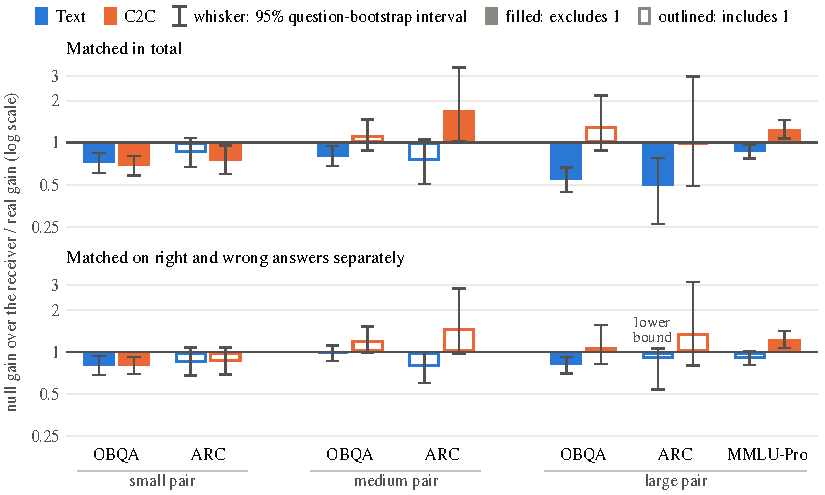
\includegraphics[width=\linewidth]{figures/figure_null_paired.pdf}
\caption{Matched one path at a time, the content-free null never falls significantly below the medium- and large-pair C2C paths, whereas whether it falls significantly below Text depends on the match: in five of seven populations unstratified and in two of six stratified. Bar: the null's gain over the receiver divided by the real path's gain (mean of 1,000 draws), drawn from 1 on a log scale, so a bar below 1 means that the null gained less than the real path; whisker: 95\% question-bootstrap interval; filled: the interval excludes 1; outlined: it includes 1. Top: unstratified; bottom: stratified. Large-pair ARC Text under the stratified match is a lower bound. Every value is in Tables~\ref{tab:null_matched} and~\ref{tab:e22}.}
\label{fig:null_paired}
\end{figure}

\paragraph{Null control.} Each receiver agent was rerun alone with its options rotated by one position (with the answer mapped back) and with the Text prompt carrying the saved helper message of another question from the same population (the question $\lfloor N/2\rfloor$ positions later in the frozen order). An unchanged rerun reproduced every receiver-only output, confirming these changes are not run-to-run noise. Option rotation changes 6.69 to 75.20\% of the receiver's answers, and another question's message changes 4.01 to 29.77\% (Table~\ref{tab:null_headroom}). Before matching, an oracle over the receiver and these two inputs achieves at least as much headroom as the oracle over $R$, Text, and C2C in six of seven populations. Text answers more questions correctly than another question's message in six of seven populations, by 1 to 30 (small-pair ARC is the exception, 126 against 130). Because an oracle gains more when more answers change, a rate-matched null action replaces $o_R(x)$ with a random differing perturbed answer on randomly drawn questions. It changes exactly as many answers as Text only ($a$), C2C only ($b$), and both jointly ($c$) (joint design; the per-reference and independent designs match one reference at a time). Ratios average 1,000 draws with 2,000-resample question bootstraps, all fixed before any of these numbers was computed. For medium ARC, the joint ratio is a lower bound due to under-matching (73 eligible questions for 77). Another question's message alone cannot serve as a rate-matched null, because it changes fewer answers than Text across all populations. When Text and C2C change a question to different answers, the two joint nulls must still agree on it if only one alternative answer exists (on average 1.0 to 133.3 questions per draw). This lowers the null gain, so the joint ratio, if anything, understates what the null reproduces.

\paragraph{Gain and headroom.} As gain over $R$, the joint null reproduces a median 76.1\% [67.6, 88.5] of the real gain (64.1 to 97.0\%), and the independent design a median 73.8\%. Matched one reference at a time, the null gains less than Text in all seven populations, but more than C2C in four. This is descriptive and does not split the real gain into a part due to content and a remainder, because real and null changes occur on different questions. Joint-null headroom over the best fixed action equals or exceeds the real one in six of seven populations (median ratio 1.149 [1.000, 1.316]; independent 1.111, Text only 1.235, C2C only 1.306). This is partly because Text outperforms $R$ by 4 to 61 questions, whereas each null action is on average below $R$ in six of seven, so $R$ remains the best fixed action of the null triple in 0.5 to 95\% of draws. Matching separately on questions $R$ answers correctly and incorrectly gives a headroom ratio of 0.967 [0.800, 1.040] (0.905 over the four populations where both strata match fully) and a gain-over-$R$ ratio of 0.849 [0.733, 0.937].

\begin{table}[!htbp]\centering\scriptsize
\caption{Rate-matched nulls without answer-specific content reproduce a median 0.761 of the real gain over $R$ and a median 1.149 of the real headroom over the best fixed action (development sets). Ratios: matched null over real (mean of 1,000 draws) [question bootstrap 95\% CI]. Best fixed action: the best single path (for the null, of $R$ and the two null actions). Joint: two nulls changing as many answers as Text only, C2C only, and both (all paths in Table~\ref{tab:complementarity_main}); Independent: one null per reference, each matched to that reference alone. (a) Real, Null: oracle gain over $R$ in questions for $\{R,\mathrm{Text},\mathrm{C2C}\}$ and for the unmatched null over $R$ and the two perturbed inputs (option rotation: each option's text moved one position down, labels kept; other message: the Text prompt carrying another question's helper message); Text, C2C: per-reference design, each reference against its own matched null (per path in Table~\ref{tab:complementarity_main}). (b) Rotated, Other message: share of $R$'s answers that rotating the options or another question's message changes; Real, Null: headroom in questions (null: joint design, mean over draws); Stratified: joint design run separately on questions $R$ answers correctly and incorrectly. $^{\dagger}$Not fully matched: in (a) the joint ratio, a lower bound; in (b) the stratified ratios (for medium ARC, all three).}
\label{tab:null_matched}\label{tab:null_headroom}\label{tab:null}
\renewcommand{\arraystretch}{1.2}\setlength{\tabcolsep}{2pt}
\vspace{5pt}\textit{(a) Gain over $R$}\par\smallskip
\begin{tabular*}{\linewidth}{@{\extracolsep{\fill}}llcrcccc@{}}\toprule
& & \multicolumn{2}{c}{\begin{tabular}[b]{@{}c@{}}Oracle gain\\(questions)\end{tabular}} & \multicolumn{4}{c@{}}{Null/real ratio [95\% CI]}\\\cmidrule(lr){3-4}\cmidrule(l){5-8}
Pair & Task & Real & \multicolumn{1}{c}{Null} & Independent & Text & C2C & Joint\\\midrule
small & OBQA & 213 & 203 & 0.686 [0.595, 0.782] & 0.719 [0.606, 0.845] & 0.686 [0.584, 0.804] & 0.664 [0.573, 0.759]\\
small & ARC & 94 & 90 & 0.738 [0.608, 0.889] & 0.851 [0.671, 1.080] & 0.747 [0.598, 0.953] & 0.737 [0.605, 0.893]\\
medium & OBQA & 103 & 106 & 0.805 [0.692, 0.937] & 0.800 [0.680, 0.945] & 1.125 [0.880, 1.464] & 0.903 [0.769, 1.048]\\
medium & ARC$^{\dagger}$ & 31 & 28 & 0.772 [0.535, 1.060] & 0.742 [0.505, 1.057] & 1.705 [1.019, 3.449] & 0.845 [0.567, 1.144]\\
large & OBQA & 53 & 62 & 0.701 [0.578, 0.856] & 0.547 [0.443, 0.665] & 1.313 [0.882, 2.175] & 0.761 [0.613, 0.935]\\
large & ARC & 12 & 9 & 0.562 [0.334, 0.803] & 0.498 [0.263, 0.778] & 0.986 [0.490, 2.970] & 0.641 [0.369, 0.900]\\
large & MMLU-Pro & 276 & 317 & 0.884 [0.800, 0.981] & 0.861 [0.769, 0.969] & 1.246 [1.071, 1.447] & 0.970 [0.877, 1.079]\\\midrule
\multicolumn{4}{@{}l}{Median over populations} & 0.738 [0.659, 0.825] & 0.742 [0.644, 0.840] & 1.125 [0.895, 1.349] & 0.761 [0.676, 0.885]\\\bottomrule
\end{tabular*}
\par\vspace{17pt}
\textit{(b) Headroom over the best fixed action}\par\smallskip
\begin{tabular*}{\linewidth}{@{\extracolsep{\fill}}llcccrcrr@{}}\toprule
& & \multicolumn{2}{c}{\begin{tabular}[b]{@{}c@{}}$R$'s answers\\changed (\%)\end{tabular}} & \multicolumn{2}{c}{\begin{tabular}[b]{@{}c@{}}Headroom\\(questions)\end{tabular}} & \multicolumn{3}{c@{}}{Null/real ratio [95\% CI]}\\\cmidrule(lr){3-4}\cmidrule(lr){5-6}\cmidrule(l){7-9}
Pair & Task & Rotated & Other message & Real & \multicolumn{1}{c}{Null} & \begin{tabular}[b]{@{}c@{}}Headroom,\\unstratified\end{tabular} & \multicolumn{1}{c}{\begin{tabular}[b]{@{}c@{}}Headroom,\\stratified\end{tabular}} & \multicolumn{1}{c@{}}{\begin{tabular}[b]{@{}c@{}}Gain over $R$,\\stratified\end{tabular}}\\\midrule
small & OBQA & 75.20 & 28.71 & 132 & 138.1 & 1.046 [0.883, 1.211] & 0.787 [0.709, 0.873] & 0.729 [0.640, 0.826]\\
small & ARC & 69.90 & 29.77 & 49 & 56.3 & 1.149 [0.922, 1.490] & 0.725 [0.592, 0.873] & 0.754 [0.626, 0.904]\\
medium & OBQA$^{\dagger}$ & 24.66 & 20.49 & 70 & 90.9 & 1.298 [0.994, 1.587] & 0.996 [0.884, 1.124] & 0.938 [0.791, 1.083]\\
medium & ARC$^{\dagger}$ & 17.73 & 12.04 & 27 & 25.6 & 0.950 [0.630, 1.405] & 0.939 [0.626, 1.126] & 0.849 [0.583, 1.058]\\
large & OBQA & 18.46 & 9.16 & 25 & 40.1 & 1.603 [1.071, 2.498] & 1.084 [0.946, 1.280] & 0.877 [0.755, 1.005]\\
large & ARC$^{\dagger}$ & 6.69 & 4.01 & 6 & 7.6 & 1.267 [0.513, 3.764] & 0.967 [0.537, 1.500] & 0.750 [0.429, 1.084]\\
large & MMLU-Pro & 34.61 & 20.26 & 239 & 260.8 & 1.091 [0.956, 1.217] & 1.023 [0.923, 1.108] & 0.956 [0.866, 1.058]\\\midrule
\multicolumn{6}{@{}l}{Median over populations} & 1.149 [1.000, 1.316] & 0.967 [0.800, 1.040] & 0.849 [0.733, 0.937]\\\bottomrule
\end{tabular*}
\end{table}

\begin{table}[!htbp]\centering\scriptsize
\caption{The per-reference null matched on right and wrong answers separately (stratified) next to the original per-reference null (unstratified), development sets. Per-reference null: a null matched to one reference alone (per path in Table~\ref{tab:complementarity_main}). Changed by reference: answers the reference changes, on questions $R$ answers correctly ($n_+$) or incorrectly ($n_-$); eligible for null: questions with a perturbed alternative. Oracle gain over $R$: real and null (null: mean of 1,000 draws). $^{\S}$Undetermined: fewer eligible wrong answers than changes; the ratio is a lower bound (0.990 rescaled to $n_-$ changes).}
\label{tab:e22}
\renewcommand{\arraystretch}{1.15}\setlength{\tabcolsep}{2.5pt}
\begin{tabular*}{\linewidth}{@{}lll@{\hspace{5pt}\extracolsep{\fill}}cccccccc@{}}\toprule
& & & \multicolumn{2}{c}{\begin{tabular}[b]{@{}c@{}}Changed by\\reference\end{tabular}} & \multicolumn{2}{c}{\begin{tabular}[b]{@{}c@{}}Eligible\\for null\end{tabular}} & \multicolumn{2}{c}{\begin{tabular}[b]{@{}c@{}}Oracle gain\\over $R$\end{tabular}} & \multicolumn{2}{c}{Null / real gain [95\% CI]}\\\cmidrule(lr){4-5}\cmidrule(lr){6-7}\cmidrule(lr){8-9}\cmidrule(l){10-11}
Pair & Task & Reference & \begin{tabular}[b]{@{}c@{}}$R$ right\\($n_+$)\end{tabular} & \begin{tabular}[b]{@{}c@{}}$R$ wrong\\($n_-$)\end{tabular} & $R$ right & $R$ wrong & Real & Null & Stratified & Unstratified\\\midrule
small & OBQA & Text & 75 & 264 & 179 & 411 & 136 & 109.19 & 0.803 [0.687, 0.940] & 0.719 [0.606, 0.845]\\
small & ARC & Text & 39 & 106 & 60 & 171 & 55 & 46.18 & 0.840 [0.680, 1.074] & 0.851 [0.671, 1.080]\\
medium & OBQA & Text & 49 & 125 & 103 & 150 & 82 & 79.46 & 0.969 [0.859, 1.115] & 0.800 [0.680, 0.945]\\
medium & ARC & Text & 21 & 31 & 32 & 41 & 25 & 19.67 & 0.787 [0.601, 1.004] & 0.742 [0.505, 1.057]\\
large & OBQA & Text & 18 & 54 & 82 & 84 & 46 & 37.24 & 0.809 [0.702, 0.924] & 0.547 [0.443, 0.665]\\
large & ARC & Text & 4 & 11 & 17 & 10 & 10 & 9.00 & 0.900$^{\S}$ [0.538, 1.056] & 0.498 [0.263, 0.778]\\
large & MMLU-Pro & Text & 129 & 432 & 288 & 827 & 166 & 148.20 & 0.893 [0.806, 1.006] & 0.861 [0.769, 0.969]\\
\addlinespace[2pt]
\multicolumn{9}{@{}l}{Median over the 7 Text populations} & 0.840 [0.769, 0.936] & \\
\midrule
small & OBQA & C2C & 66 & 284 & 179 & 411 & 147 & 117.72 & 0.801 [0.694, 0.923] & 0.686 [0.584, 0.804]\\
small & ARC & C2C & 24 & 136 & 60 & 171 & 69 & 59.08 & 0.856 [0.691, 1.078] & 0.747 [0.598, 0.953]\\
medium & OBQA & C2C & 48 & 83 & 103 & 150 & 44 & 52.83 & 1.201 [0.984, 1.517] & 1.125 [0.880, 1.464]\\
medium & ARC & C2C & 25 & 23 & 32 & 41 & 10 & 14.75 & 1.475 [0.964, 2.844] & 1.705 [1.019, 3.449]\\
large & OBQA & C2C & 35 & 25 & 82 & 84 & 16 & 17.24 & 1.077 [0.823, 1.558] & 1.313 [0.882, 2.175]\\
large & ARC & C2C & 6 & 6 & 17 & 10 & 4 & 5.41 & 1.351 [0.800, 3.151] & 0.986 [0.490, 2.970]\\
large & MMLU-Pro & C2C & 204 & 552 & 288 & 827 & 155 & 189.48 & 1.222 [1.067, 1.406] & 1.246 [1.071, 1.447]\\
\addlinespace[2pt]
\multicolumn{9}{@{}l}{Median over the 7 C2C populations} & 1.201 [0.947, 1.331] & \\
\multicolumn{9}{@{}l}{Median over the 5 medium- and large-pair C2C populations} & 1.222 [1.059, 1.448] & \\\bottomrule
\end{tabular*}
\end{table}

\begin{table}[!htbp]\centering\scriptsize
\caption{Direction of the changes, development sets. For each path: its changes on questions $R$ answers incorrectly (to right, to another wrong answer, and the share that become right) and on questions $R$ answers correctly (to wrong). $g_-$: expected share of a null change on a wrong answer that becomes right. (a) The two references; (b) the two perturbed inputs (option rotation: each option's text moved one position down, labels kept; other question's message: the Text prompt carrying another question's helper message).}
\label{tab:e22dir}
\renewcommand{\arraystretch}{1.15}\setlength{\tabcolsep}{2.5pt}
\vspace{5pt}\textit{(a) References}\par\smallskip
\begin{tabular*}{\linewidth}{@{}ll@{\hspace{5pt}\extracolsep{\fill}}ccccccccc@{}}\toprule
& & & \multicolumn{4}{c}{Text} & \multicolumn{4}{c}{C2C}\\\cmidrule(lr){4-7}\cmidrule(l){8-11}
& & Null share & \multicolumn{3}{c}{$R$ wrong} & $R$ right & \multicolumn{3}{c}{$R$ wrong} & $R$ right\\\cmidrule(lr){4-6}\cmidrule(lr){7-7}\cmidrule(lr){8-10}\cmidrule(l){11-11}
Pair & Task & right ($g_-$) & $\to$right & $\to$wrong & share right & $\to$wrong & $\to$right & $\to$wrong & share right & $\to$wrong\\\midrule
small & OBQA & 0.414 & 136 & 128 & 0.515 & 75 & 147 & 137 & 0.518 & 66\\
small & ARC & 0.436 & 55 & 51 & 0.519 & 39 & 69 & 67 & 0.507 & 24\\
medium & OBQA & 0.637 & 82 & 43 & 0.656 & 49 & 44 & 39 & 0.530 & 48\\
medium & ARC & 0.634 & 25 & 6 & 0.806 & 21 & 10 & 13 & 0.435 & 25\\
large & OBQA & 0.690 & 46 & 8 & 0.852 & 18 & 16 & 9 & 0.640 & 35\\
large & ARC & 0.900 & 10 & 1 & 0.909 & 4 & 4 & 2 & 0.667 & 6\\
large & MMLU-Pro & 0.343 & 166 & 266 & 0.384 & 129 & 155 & 397 & 0.281 & 204\\\bottomrule
\end{tabular*}
\par\vspace{17pt}
\textit{(b) Perturbed inputs}\par\smallskip
\begin{tabular*}{\linewidth}{@{}ll@{\hspace{5pt}\extracolsep{\fill}}ccccccccc@{}}\toprule
& & & \multicolumn{4}{c}{Rotated options} & \multicolumn{4}{c}{Other question's message}\\\cmidrule(lr){4-7}\cmidrule(l){8-11}
& & Null share & \multicolumn{3}{c}{$R$ wrong} & $R$ right & \multicolumn{3}{c}{$R$ wrong} & $R$ right\\\cmidrule(lr){4-6}\cmidrule(lr){7-7}\cmidrule(lr){8-10}\cmidrule(l){11-11}
Pair & Task & right ($g_-$) & $\to$right & $\to$wrong & share right & $\to$wrong & $\to$right & $\to$wrong & share right & $\to$wrong\\\midrule
small & OBQA & 0.414 & 164 & 235 & 0.411 & 159 & 78 & 88 & 0.470 & 47\\
small & ARC & 0.436 & 65 & 92 & 0.414 & 52 & 38 & 33 & 0.535 & 18\\
medium & OBQA & 0.637 & 66 & 43 & 0.606 & 74 & 66 & 37 & 0.641 & 49\\
medium & ARC & 0.634 & 19 & 14 & 0.576 & 20 & 16 & 7 & 0.696 & 13\\
large & OBQA & 0.690 & 48 & 23 & 0.676 & 66 & 31 & 13 & 0.705 & 24\\
large & ARC & 0.900 & 6 & 0 & 1.000 & 14 & 7 & 1 & 0.875 & 4\\
large & MMLU-Pro & 0.343 & 232 & 454 & 0.338 & 228 & 151 & 257 & 0.370 & 127\\\bottomrule
\end{tabular*}
\end{table}

\paragraph{Matching one path at a time, on right and wrong answers separately.} After the main results, under rules fixed before computing (post hoc), we evaluated the per-reference design by matching the reference's change rate separately on questions $R$ answers correctly ($S^+$) and incorrectly ($S^-$), then pooling the two draws. Because only changes on $S^-$ affect the gain over $R$, this stratified ratio equals the share of changed wrong answers that the null turns right (denoted $g_-$) divided by the reference's share (Table~\ref{tab:e22dir}). If $S^-$ contains fewer eligible questions than the reference changes, the cell is undetermined and its ratio serves as a lower bound. Intervals follow the prior protocol (2,000 resamples, 100 draws each, seed 0). As detailed in Table~\ref{tab:e22}, Text's ratio is below 1 in all six determined populations, with the interval below 1 in two (small-pair and large-pair OBQA). The large-pair ARC setting is undetermined (0.900, or 0.990 after rescaling to the reference's count). The five medium- and large-pair C2C ratios range from 1.077 to 1.475; none has an interval below 1, and the interval for large-pair MMLU-Pro exceeds 1. A prespecified Monte Carlo check (mean null gain deviating by more than three standard errors from $\min(n_-,\mathrm{elig}_-)\,g_-$) flagged medium/ARC/C2C at 3.28 standard errors. A diagnostic across 400 seeds found no systematic bias (mean deviation $-0.026$ standard errors), and seed 0 was the most extreme of the 400. After observing all results, we lifted the stop and report the prespecified numbers unchanged. This analysis reveals the direction of every change (Table~\ref{tab:e22dir}): relative to $g_-$, the share of changed wrong answers that become right differs by $+0.9$ to $+17.2$ points for Text, $-23.3$ to $+10.4$ for C2C, $-5.8$ to $+10.0$ for rotated options, and $-2.5$ to $+9.9$ for another question's message across the seven populations.

\paragraph{Overlap, confidence, and which path is right.} Each path is uniquely correct on certain questions (Figure~\ref{fig:null_sources}(a)). Text and C2C change the same questions 1.3 to 6.6 times as often as independent changes at their rates would (Figure~\ref{fig:null_sources}(b)). Both references mostly change answers when the receiver is unsure: 0 to 40.4\% of changed answers have an uncertainty $u$ at or below the fit-split median, against 45.5 to 72.6\% of all questions. For the medium pair, 14.9 and 26.9\% of Text's changes are at or below it, compared to 5.3 and 2.1\% of C2C's changes (Figure~\ref{fig:null_sources}(c)). Where exactly one of Text and C2C is right on the medium pair (155 OBQA questions, 96 with Text right; 53 ARC questions, 36 with Text right), ProbeMax separates the two with AUROC 0.569 [0.472, 0.667] (OBQA) and 0.608 [0.438, 0.753] (ARC), with bootstrap resamples stratified by class. Since both intervals include 0.5, this descriptive check establishes no signal for which path is right. Small- and medium-pair MMLU-Pro headroom is in Appendix~\ref{app:mmlu}.

\begin{figure}[!htbp]\centering
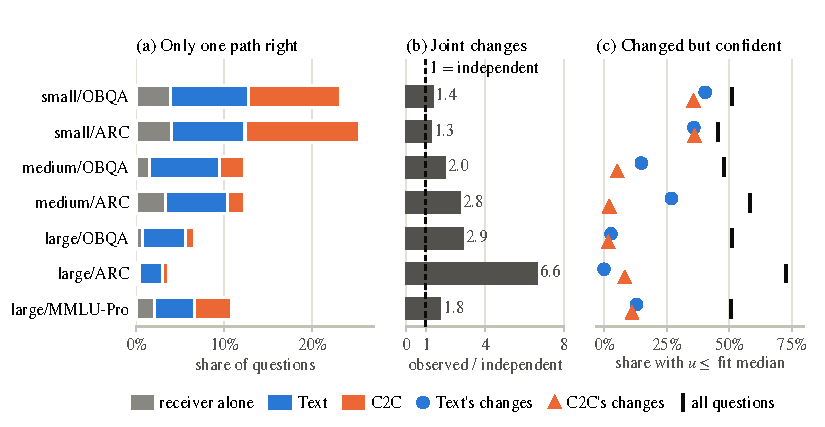
\includegraphics[width=\linewidth]{figures/figure_null_sources.pdf}
\caption{Each path is the only one right on some questions, the two references change largely the same questions, and both mostly change answers on which the receiver is unsure (development sets). (a) Questions that only the receiver alone, only Text, or only C2C answers correctly, as a share of the population. (b) Questions changed by both references, divided by the number that independent changes at the observed rates would give. (c) Share of the answers each reference changes whose receiver uncertainty $u$ is at or below the fit-split median; tick: share of all questions.}
\label{fig:null_sources}
\end{figure}
